\begin{abstract}
The closing chapter brings together two different structures: a line-of-sight accumulation law with saturation $1/\pi$, and a matter-inventory assignment with the same numerical value. Their equality is exact within the declared count rules, but a cosmological future requires a time-evolution law and a calibrated observable. We distinguish a distance-fit coefficient from the fractional expansion rate, derive the conditions under which the original $\Omega_\Lambda^{3/2}$ expression is meaningful, and formulate finite-redshift tests. The completed-boundary or Home continuation is then developed as an explicit conditional ledger, with conservation, radius-floor and information-channel requirements. A worked receipt sequence demonstrates growth while emitting, and a differential distance test exposes the assumptions hidden in a simple rate rescaling. The resulting closure program connects the thermal boundary, radiation response and cosmological inventory without treating their common numerical factors as a substitute for dynamics. No transition mechanism or future cosmological solution is claimed to have been established by count identities alone.
\end{abstract}

\section{The two arcs that meet at the end of the volume}
Volume I begins with a floor and a source-induced lift. The floor supplies a reference level; the lift describes an accumulation attributed to a particular source. Chapters III--VII follow the source coordinate toward a completed boundary and ask how clocks, records, fields and thermal exchange behave there. Chapters VIII--X use the floor in a proposed cosmic inventory and in the organization of many-source systems. Chapter XI asks whether the released carrier account can become an independently testable radiation law.

The original ending joins these arcs in two ways. First, it identifies the limiting line-of-sight road accumulation with the matter fraction. Second, it proposes that a completed Home can supply a new floor through a change of informational indexing. Both are substantial ideas. Neither should be weakened by asking a numerical identity to establish a causal process that has not yet been specified.

This chapter therefore keeps the original proposals while separating four levels of statement. An identity follows from the chosen counts. A conditional theorem follows after its physical premises are declared. An adapter imports a conventional geometry or evolution law. A conjecture identifies a possible continuation whose mechanism remains to be found. The end of the volume is strongest when these levels remain visible, because they show exactly which result a future calculation would add.

The word ``fate'' also requires care. The future of a cosmological solution is a statement about evolution in proper time. The saturation of an integral along the present past light cone is a statement about progressively more distant emission events. A change of radial distance convention is yet another operation. The three can be related by a theory, but they cannot be interchanged by notation.

\section{The road law and what it actually proves}
For the nonnegative redshift domain of the original proposal, define
\begin{equation}
 A_{\rm los}(z)=A_0R\left[1-(1+z)^{-\widehat d}\right]
 =\frac1\pi\left[1-(1+z)^{-3}\right],\qquad z\geq0.
 \label{c12:road}
\end{equation}
The model uses $A_0R=1/\pi$ and $\widehat d=3$. Direct differentiation gives
\begin{equation}
 \frac{dA_{\rm los}}{dz}=\frac3\pi(1+z)^{-4}>0,
 \qquad
 \frac{d^2A_{\rm los}}{dz^2}=-\frac{12}\pi(1+z)^{-5}<0.
 \label{c12:roadderivatives}
\end{equation}
Thus the road starts at zero, initially rises with slope $3/\pi$, is monotone and concave, and has the exact limit $1/\pi$. Its survival factor is
\begin{equation}
 f(z)=1-A_{\rm los}(z)=1-\frac1\pi+\frac1{\pi(1+z)^3}.
 \label{c12:survival}
\end{equation}
For $z\geq0$, $1-1/\pi<f(z)\leq1$. No dynamics is needed to prove these statements. They are properties of the proposed function, not yet a derivation of that function from microscopic transport.

At small redshift the expansions are
\begin{align}
 A_{\rm los}(z)&=\frac1\pi\left(3z-6z^2+10z^3+O(z^4)\right),
 \label{c12:roadseries}\\
 f(z)&=1-\frac{3z}{\pi}+\frac{6z^2}{\pi}+O(z^3).
 \label{c12:fseries}
\end{align}
These coefficients are more directly testable than an asymptotic number, once the road is connected to an observable. At $z=1$, for example, the proposed accumulation is $7/(8\pi)$ and the survival factor is about $0.7215$. Any interpretation that changes a measured distance by this factor has a substantial finite-redshift consequence. It cannot be defended solely by noting that its limiting value resembles a cosmological inventory fraction.

There is a useful alternative variable for the mathematical road. Let $u=\log(1+z)$. Then $A_{\rm los}=(1-e^{-3u})/\pi$ and
\begin{equation}
 \frac{dA_{\rm los}}{du}=3\left(\frac1\pi-A_{\rm los}\right).
 \label{c12:roadode}
\end{equation}
This is an exact differential representation of the supplied curve. It is not a future-time relaxation law: $u$ labels lookback redshift along a specified observation cone. Treating it as a clock would add a new identification and must be justified independently.

\section{Equal numbers, different operators}
The inventory assignment of Chapter VIII is
\begin{equation}
 \Omega_{m,*}=RA_0=\frac1\pi,\qquad
 \Omega_{\Lambda,*}=1-\Omega_{m,*}=\frac{\pi-1}{\pi}.
 \label{c12:inventory}
\end{equation}
An asterisk emphasizes that these are the clean count-assigned fractions before corrections or additional present-day components are specified. The original typed join is then
\begin{equation}
 A_{\rm los}(\infty)=\Omega_{m,*},\qquad
 f(\infty)=\Omega_{\Lambda,*}.
 \label{c12:typedjoin}
\end{equation}
The equality is exact as a consequence of the common input $RA_0$. It does not prove that the road operator measures matter density, or that its complement has negative pressure. An inventory is a weight assigned to sectors of a state. A propagation observable is an operation on a source, path, detector and calibration. Equal expectation values do not make those operations identical.

A stronger version of the join would start with a normalized preparation measure $\mu$ on actual source states and two declared observables, $\mathcal I_m$ and $\mathcal R_{\rm los}$. It would show
\begin{equation}
 \int \mathcal I_m\,d\mu=\frac1\pi,
 \qquad
 \lim_{z\to\infty}\int\mathcal R_{\rm los}(z)\,d\mu=\frac1\pi,
 \label{c12:operatorjoin}
\end{equation}
with both normalizations derived from the same preparation and no target-dependent adjustment. This is the source-measure interface identified in the closing review. It would replace a numerical coincidence within a grammar by a common physical cause.

The component accounting also has to close. If a spatially flat present-day Friedmann adapter includes a nonzero radiation density, then $1=\Omega_{r,0}+\Omega_{m,0}+\Omega_{\Lambda,0}$. Assigning both fractions in \eqref{c12:inventory} exactly while adding radiation makes their sum exceed one. One may work in a late-time approximation neglecting radiation, assign $\Omega_{\Lambda,0}=1-\Omega_{m,0}-\Omega_{r,0}$, or change the definition of the clean ledger. The choice must be explicit. A small correction is still a correction when the proposal claims exactness.

\section{The background adapter and its conditional late-time limit}
The original fate calculation adopts
\begin{equation}
 H^2(a)=H_0^2\left(\Omega_{r,0}a^{-4}
              +\Omega_{m,0}a^{-3}+\Omega_{\Lambda,0}\right),
 \label{c12:friedmann}
\end{equation}
with $a=1$ today and a consistent normalization of its coefficients. This is a flat radiation--matter--cosmological-constant adapter. It assumes the relevant conservation laws, an expanding branch, and a positive constant vacuum term. Under those assumptions, the dilution terms vanish as $a\to\infty$ and
\begin{equation}
 H_{\infty,\rm native}=H_0\sqrt{\Omega_{\Lambda,0}}.
 \label{c12:hinfinity}
\end{equation}
The conclusion is valid conditional mathematics, but it inherits the cosmological-constant behavior from the adapter. An inventory complement has not independently derived that behavior.

The approach can also be quantified. Factoring out $\Omega_{\Lambda,0}$ and expanding the square root gives
\begin{equation}
 \frac{H(a)}{H_0\sqrt{\Omega_{\Lambda,0}}}
 =1+\frac{\Omega_{m,0}}{2\Omega_{\Lambda,0}}a^{-3}
   +\frac{\Omega_{r,0}}{2\Omega_{\Lambda,0}}a^{-4}+O(a^{-6}).
 \label{c12:approach}
\end{equation}
Along the expanding branch, the limiting equation $\dot a/a=H_{\infty,\rm native}$ has exponential solutions. This establishes the late-time behavior of the stated adapter; it does not establish stability against arbitrary changes of the source theory or additional components.

For a component with equation of state $p=w(a)\rho c^2$, separate conservation would instead give
\begin{equation}
 \rho(a)=\rho(1)\exp\left[-3\int_1^a(1+w(\widetilde a))
                                      \,d\log\widetilde a\right].
 \label{c12:darkenergy}
\end{equation}
A constant density follows only when $w=-1$, or when a separately specified exchange compensates its evolution. If the Home population feeds an effective background, that exchange must appear in the continuity equations. A successful mechanism might derive it, but the number $(\pi-1)/\pi$ alone contains no pressure, transfer rate or stability information.

Measurements such as Planck's parameter inference and DESI's distance constraints are relevant comparators [XII.1, XII.2]. They do not measure a count identity directly: they constrain an evolution and observation model. Consequently, agreement of an adopted present-day density fraction with one parameter fit does not settle the cosmological future, and a model-specific tension should not be quoted without the exact data combination and likelihood assumptions.

\section{Past-cone saturation is not future-time saturation}
In an ordinary homogeneous cosmological chart, redshift relates an emission scale factor to the observer's scale factor through $1+z=a(t_o)/a(t_e)$. Keeping $t_o$ fixed while taking $z\to\infty$ sends the emission time toward the early universe. It does not send the observer to the future. If one sets $a(t_o)=1$ and mechanically substitutes $1+z=1/a$ into \eqref{c12:road}, one obtains
\begin{equation}
 A_{\rm los}=\frac1\pi(1-a^3).
 \label{c12:badextension}
\end{equation}
For $a>1$ this becomes negative and tends to minus infinity. The substitution is a useful diagnostic: the supplied past-cone function is not a nonnegative future saturation law on that domain.

A cosmological road should instead carry its arguments explicitly. One possible notation is $A_{\rm los}(t_o,t_e,\mathcal P)$, where $\mathcal P$ identifies the ray or route and the preparation of the medium. A homogeneous effective road might depend on an integral of a rate along the ray,
\begin{equation}
 A_{\rm los}=\mathcal F\!\left(\int_{t_e}^{t_o}
                        \Gamma(t,\mathcal P)\,dt\right),
 \label{c12:roadfunctional}
\end{equation}
but the rate, saturation function and conservation law must come from the model. Writing an integral does not by itself identify the microscopic carriers or show that their accumulation is positive.

The future limit also needs a family of observations. Does the observer follow a fixed comoving source, a fixed proper-distance source, a fixed emission-time surface, or the edge of an accessible region? Each family changes the relation among $t_o$, $t_e$ and distance. A single number called the ``remaining road'' is insufficient until that family and its clocks are chosen.

As a mathematical example only, a future variable $B(N)$ with $N=\log a$ could obey $dB/dN=\lambda(B_*-B)$ for $\lambda>0$. Then $B=B_*+[B(0)-B_*]e^{-\lambda N}$, so $B_*$ is an attractor. Choosing $B_*=1/\pi$ reproduces the desired limit but does not derive it. This toy equation identifies the missing tasks: derive the fixed point, the sign and magnitude of its relaxation, the physically allowed interval and the source of any dissipated energy.

\section{The fate coefficient and the meaning of an expansion rate}
The working draft uses
\begin{equation}
 D_{\rm native}=fD_{\rm readout}
 \label{c12:distancemap}
\end{equation}
and proposes multiplication of the background rate by $f_\infty$. There is one clear operational situation where that multiplication is correct. If a separately fixed velocity-like numerator obeys $v=H_{\rm native}D_{\rm native}$ and one fits the same numerator against $D_{\rm readout}$, then
\begin{equation}
 H_{\rm fit}\equiv\frac{v}{D_{\rm readout}}
              =fH_{\rm native}.
 \label{c12:fitrate}
\end{equation}
Assuming additionally that a future observing family has $f_\infty=\Omega_{\Lambda,*}$, and using the radiation-neglecting adapter, this gives the original expression
\begin{equation}
 H_{{\rm fit},\infty}=H_0\Omega_{\Lambda,*}^{3/2}
 =H_0\left(\frac{\pi-1}{\pi}\right)^{3/2}
 \simeq0.562834H_0.
 \label{c12:conditionalfate}
\end{equation}
This is a conditional distance-fit coefficient. The numerator, clock and calibration must remain fixed exactly as stipulated. At cosmological distances, recession velocity is not generally a directly measured local velocity, so the observation rule cannot be left implicit.

A fractional expansion rate behaves differently. For a comoving separation $D_{\rm native}=a\chi$ with fixed $\chi$, differentiating \eqref{c12:distancemap} using the same time coordinate yields
\begin{equation}
 \frac{\dot D_{\rm readout}}{D_{\rm readout}}
 =H_{\rm native}-\frac{\dot f}{f}.
 \label{c12:fractionalrate}
\end{equation}
If $f$ approaches a nonzero constant and $\dot f/f\to0$, this rate approaches $H_{\rm native}$, not $f_\infty H_{\rm native}$. A constant rescaling of distance cancels from a logarithmic derivative. This simple identity is essential to the final claim: the original multiplication cannot be described as a future Hubble rate without an operational definition that differs from the usual fractional expansion rate.

Changing the clock would add another factor. If $dt_{\rm readout}=g(t)dt$, then the measured fractional rate becomes $[H_{\rm native}-\dot f/f]/g$. Neither $g$ nor its asymptote follows from a distance fraction. Chapter IV's local invariant light speed is compatible with many coordinate or readout conventions; it does not select one of them. The calibration of clocks, rulers and propagation must be supplied together.

\begin{figure*}[t]
\centering
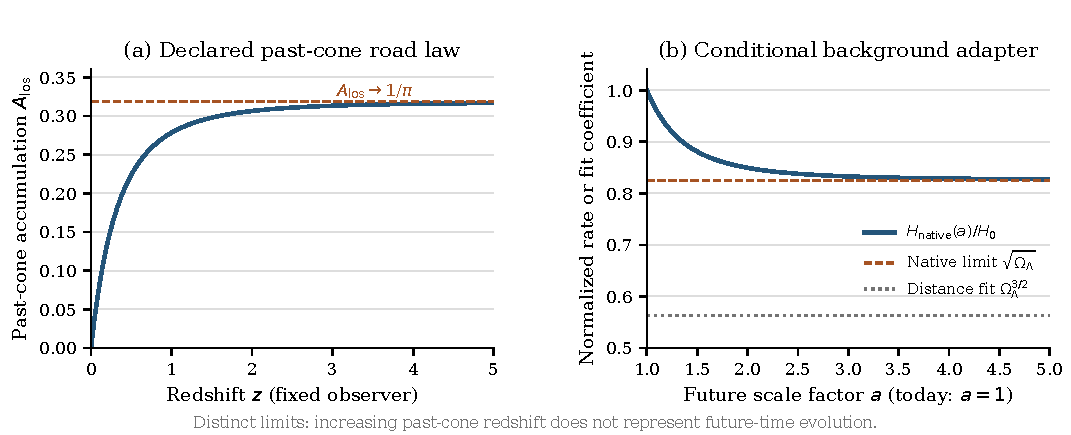
\includegraphics[width=\textwidth]{figures/ch12_distinct_limits.pdf}
\caption{Two mathematically distinct limits. (a) The declared past-cone road law $A_{\rm los}(z)=\pi^{-1}[1-(1+z)^{-3}]$ approaches $1/\pi$ as redshift increases for a fixed observer. (b) With radiation neglected, $\Omega_m=1/\pi$ and $\Omega_\Lambda=1-1/\pi$, the adopted flat matter--constant-vacuum adapter gives $H_{\rm native}(a)/H_0=\sqrt{\Omega_m a^{-3}+\Omega_\Lambda}$ and tends to $\sqrt{\Omega_\Lambda}$. The lower dotted reference, $\Omega_\Lambda^{3/2}$, is a conditional distance-fit coefficient, not the native fractional-expansion limit; it requires the additional future observing-family and calibration assumptions in the text. Past-cone saturation does not derive a future road limit. These curves are analytic illustrations of declared premises, not observational data or an independently derived SAM future.}
\label{fig:c12:limits}
\end{figure*}

\section{Numerical values with an honest uncertainty ledger}
Using the original clean fractions and the frozen Chapter VIII value $H_{0,\rm SAM}=67.2504\ {\rm km\,s^{-1}\,Mpc^{-1}}$, the native adapter limit is approximately $55.525$ in the same units and the conditional fit coefficient is approximately $37.851$. The original alternatives $H_0=68.76$ and $73.04$ give conditional fit values about $38.700$ and $41.109$. These are rescalings of a selected input, not three independent confirmations of the theory.

The exact dimensionless expression is more portable than any one dimensional value. Even so, its apparent exactness does not remove uncertainty in the choice of inventory, the road interpretation or the dynamical adapter. If $F=H_0\Omega_\Lambda^{3/2}$, first-order propagation of continuous input errors gives
\begin{equation}
 \frac{\delta F}{F}=\frac{\delta H_0}{H_0}
                  +\frac32\frac{\delta\Omega_\Lambda}{\Omega_\Lambda}.
 \label{c12:errorlinear}
\end{equation}
A variance calculation must preserve the covariance of the inputs. Structural alternatives, such as a different road operator or a nonconstant dark-energy equation of state, are not captured by this linear formula. They require separate model branches.

The closing review cautions that the small propagated temperature uncertainty in the Hubble cascade is not a total theory uncertainty. This chapter adopts that caution. A conditional number may be computed to many decimal places, but the number of printed digits should not imply that discrete choices, calibration assumptions and uncomputed source corrections are known to that precision.

\section{Finite-redshift observations and distance duality}
A useful road theory must say which distances change. In a metric description with photon number conservation and null-geodesic propagation, luminosity and angular-diameter distances obey
\begin{equation}
 D_L=(1+z)^2D_A.
 \label{c12:duality}
\end{equation}
The physical assumptions behind this relation matter more than its use as a convenient identity. Distance-duality tests compare different measurement channels and can reveal an inconsistency in an assigned propagation factor [XII.3].

Suppose a proposed readout changes the two distances by factors $g_L(z)$ and $g_A(z)$ relative to a common metric adapter. Then the diagnostic ratio is
\begin{equation}
 \eta_D(z)=\frac{D_{L,\rm readout}}{(1+z)^2D_{A,\rm readout}}
          =\frac{g_L(z)}{g_A(z)}.
 \label{c12:dualityratio}
\end{equation}
If only luminosity distance is multiplied by $1/f$, then $\eta_D=1/f$. If both distances receive the same factor, the ratio remains one. Thus a road factor is not automatically a distance-duality violation, contrary to an overly broad reading of the closing review. The violation depends on the observation map. A common rescaling still affects other distance and expansion comparisons and is not automatically viable.

For a concrete differential test, assume a flat adapter with $D_C(z)=c\int_0^z dz'/H(z')$, and apply $D_{C,\rm readout}=D_C/f$. An analyst interpreting this new distance by the same integral relation would infer
\begin{equation}
 H_{\rm inferred}(z)
 =\frac{c}{d(D_C/f)/dz}
 =\frac{H(z)f(z)^2}
 {f(z)-[H(z)D_C(z)/c]f'(z)}.
 \label{c12:inferredH}
\end{equation}
This is not simply $fH$. The derivative of the road contributes. At $z=0$, $D_C=0$ and $f=1$, so this particular map preserves the local intercept $H_0$ while changing higher-order distance behavior.

The same point appears in a small-redshift expansion. If $q_0$ is the adapter deceleration parameter, $D_C=(c/H_0)[z-(1+q_0)z^2/2+O(z^3)]$. Dividing by \eqref{c12:fseries} and fitting the same form gives
\begin{equation}
 q_{0,\rm inferred}=q_0-\frac6\pi.
 \label{c12:qshift}
\end{equation}
The shift is large. It is a falsifiable consequence of this particular uncompensated distance map, not a claim that all possible SAM road operators predict it. A viable alternative must explicitly show which other calibration or geometry factors compensate it; silently canceling the factor would erase the claimed new observable.

\section{A completed Home: retained proposal and conditional closure}
The second arc of the original chapter describes a Home as a closed two-dimensional ledger with an interior side and a parent-domain exterior side. Apparent bulk volume is interpreted as ordered information on the surface, rather than an additional ontic three-dimensional interior. Tagged child histories retain their custody under recursive maps. These are organizing postulates of the Home proposal, not deductions from the Schwarzschild metric.

The original lifecycle has three stages. A pre-completion collapse state has no filled point interior; localization remains assigned to the forming surface. During formation, the origin-matter lane and the captured outside-origin baryon lane establish a formation inventory. At completion, the source coordinate reaches $A=1$ and the ledger is sealed under the proposed crossing rule. The historical identifiers H000791 and H000794--H000797 record this construction.

Chapter V already limits how strongly the last step may be stated. Its source coordinate satisfies $A(r_s)=1$; this is not the condition $A_0+A=1$. Its finite-impulse and finite-distance results depend on the source law. In the relevant infinite-approach route, a calculated source satisfying the radial null-energy condition is screened by the theorem; otherwise the actual energy-condition violation or flux must be propagated. Chapter XII cannot turn this conditional result into an unconditional physical law of infinite crossing cost.

Accordingly, the completed Home account below is conditional on a source-selected completion dynamics and boundary law consistent with Chapter V. It may impose an empty post-completion crossing relation as part of that model, but must then derive the stress, work and causal response that realize it. Coordinate-time delay in a Schwarzschild exterior does not by itself establish infinite local crossing cost. The physical statement requires an operational trajectory and energy account.

\section{Exterior balance and the radius floor}
Once the conditional completion is stipulated, define $M_{\rm form}>0$ as the frozen formation inventory and $E_n\geq0$ as a mutable exterior mass-equivalent inventory. Let $I_n,O_n\geq0$ be realized incoming and outgoing mass-equivalent receipts over step $n$. The proposed recurrence is
\begin{equation}
 \begin{gathered}
 E_{n+1}=E_n+I_n-O_n,\qquad 0\leq O_n\leq E_n+I_n,\\
 M_n=M_{\rm form}+E_n.
 \end{gathered}
 \label{c12:recurrence}
\end{equation}
The explicit upper bound on $O_n$ is what preserves nonnegativity. If $E_0\geq0$, induction gives $E_n\geq0$ for every subsequent step. Summing the recurrence gives the exact cumulative identity
\begin{equation}
 E_N=E_0+\sum_{n=0}^{N-1}I_n-\sum_{n=0}^{N-1}O_n,
 \qquad
 \sum O_n\leq E_0+\sum I_n.
 \label{c12:cumulative}
\end{equation}
These are ledger theorems. They do not specify a physical emission rate or show that every allowed sequence occurs.

If the Schwarzschild mass--radius adapter is adopted at each quasi-static step,
\begin{equation}
 R_n=\frac{2G(M_{\rm form}+E_n)}{c^2},\qquad
 R_{\rm form}=\frac{2GM_{\rm form}}{c^2},
 \label{c12:radius}
\end{equation}
then $R_n\geq R_{\rm form}$. An area-based record count with fixed area per unit satisfies
\begin{equation}
 \frac{N_n}{N_{\rm form}}=
 \left(\frac{R_n}{R_{\rm form}}\right)^2
 =\left(1+\frac{E_n}{M_{\rm form}}\right)^2\geq1.
 \label{c12:areamemory}
\end{equation}
This consequence requires both the adapter and an unchanged microscopic area unit. If the completion mechanism alters either, the area-memory formula must be rederived.

A worked example clarifies gross output versus net change. In arbitrary mass units choose $M_{\rm form}=10$ and $E_0=2$. An interval with $I_0=3$ and $O_0=1$ ends at $E_1=4$: the Home emits while its total mass grows from 12 to 14. Next take $I_1=0$ and $O_1=3$, obtaining $E_2=1$ and total mass 11. Finally $I_2=0$, $O_2=1$ exhausts the exterior account and leaves the floor 10. The cumulative output is 5, paid by initial exterior inventory 2 plus inflow 3. At no step is the formation floor debited.

A positive floor has a sharp thermodynamic consequence. If all incoming supply ceases and exterior inventory drains, the proposed output must eventually cease or change its law. A temperature formula by itself cannot authorize continued emission from a frozen reservoir. The boundary transition strengths and available states must implement the floor. This is where Chapter VII's thermal account must meet the lifecycle rather than remain a separate analogy.

\section{Continuous evolution, vacuum exteriors and surface response}
A continuum approximation to the recurrence is
\begin{equation}
 \dot E=\dot M_{\rm in}-\dot M_{\rm out},\qquad E\geq0.
 \label{c12:continuous}
\end{equation}
At $E=0$, the boundary rule must prevent $\dot M_{\rm out}>\dot M_{\rm in}$. A formal ordinary differential equation that continues to negative $E$ violates the model's own domain. One can impose a constrained flow, but a microscopic theory should explain its origin through allowed transitions and detailed energy payments.

There is also a geometry requirement. A spherically symmetric vacuum exterior in general relativity has a constant Schwarzschild mass parameter locally; time-varying mass caused by actual inflow or radiation requires nonvacuum stress in the relevant region [XII.4]. Therefore \eqref{c12:radius} is at most an instantaneous or quasi-static adapter during exchange. It is not a complete spacetime solution for arbitrary receipt sequences. Matching an emitting surface to its exterior requires the energy flux and junction conditions.

The same surface cannot be assigned independently chosen optical, thermal and gravitational-wave properties. A hard reflective surface, a dissipative membrane and an absorbing horizon can share an approximate exterior mass profile while having different responses. Chapter XI's impedance and Chapter VII's thermal transitions must be compatible with the Home custody rules. A boundary that stores a pulse must say where its energy goes and how a later receipt releases it. A boundary that permanently hides information must specify the channel seen by each side.

These obligations also prevent a purely semantic resolution of the singularity question. Calling the boundary an information surface does not calculate its stress or establish a nonsingular evolution. Conversely, a successful surface model would not need a classical bulk interpretation to be meaningful if it provided a consistent state space, dynamics, observation map and tested exterior limit. Those are the appropriate requirements for the proposal on its own terms.

\section{Quantum custody and what an exterior observer can learn}
The original Home rules describe unresolved horizon matter as unavailable to either side. A failed incoming attempt retains its exterior receipt; a retained post-completion receipt has a finite sequence of attempted inward operations followed by a realized outward operation. The terminal outward receipt debits scalar parent-visible mass. This is a proposed event grammar, not yet a Hamiltonian or a quantum instrument.

A physical version can represent an allowed step by an instrument $\{\mathcal E_r\}$ indexed by receipts $r$. Each map is completely positive and trace nonincreasing; their sum is trace preserving when all outcomes are included. Probabilities are $p_r=\operatorname{Tr}\mathcal E_r(\rho)$, and conditioned states are $\mathcal E_r(\rho)/p_r$. Conservation then requires the mean receipt energies and changes in source, surface and control energy to agree. Naming an outcome ``OUT'' does not supply this equality.

The assertion that each receipt eventually exits also needs a precise quantifier. Every member of a finite set may have a finite exit schedule, yet an indefinitely replenished population need not empty at any finite time. A stochastic model can have eventual exit with probability one while having an infinite mean waiting time. Neither a uniform finite completion time nor a finite luminosity follows from individual eventual realization. The waiting-time distribution is part of the observable dynamics.

The parent-facing scalar quotient severely limits accessible information. If two internal states $\rho$ and $\sigma$ induce the same output channel state, no measurement on that output distinguishes them. More generally, a completely positive trace-preserving channel $\Phi$ contracts trace distance,
\begin{equation}
 \frac12\|\Phi(\rho)-\Phi(\sigma)\|_1
 \leq\frac12\|\rho-\sigma\|_1.
 \label{c12:contraction}
\end{equation}
This is the operational frame already used in Chapter VI. A child history that never changes any allowed parent output is not parent-observable. A proposed test must identify which output distribution, response function or conserved scalar actually depends on the child data.

Preserving custody is also different from duplicating an arbitrary quantum state. Side tags and ancestry labels may record classical provenance, but a coherent state cannot be copied freely into independently readable ledgers. The Home map must specify whether it is an isometry, a coarse-graining channel, a conditional instrument or some other well-defined transformation, and carry correlations with the environment accordingly.

\section{Re-indexing a completed boundary into a new floor}
The original handoff identity is
\begin{equation}
 A_0=\frac{A_H}{4\pi D},
 \label{c12:handoff}
\end{equation}
where $A_H$ is the unit completion value in the relevant normalization and $D$ is the spatial-dimension count. To avoid confusion with physical distances elsewhere in this chapter, write $D_{\rm count}=3$ here. With $A_H=1$ and $R=4D_{\rm count}=12$, the identity yields $A_0=1/(12\pi)$ and $RA_0=1/\pi$. The independence of the product from $D_{\rm count}$ holds only when the relation $R=4D_{\rm count}$ is retained.

The arithmetic is clear; the direction and mechanism of the handoff need more definition. The working chapter alternates between a child floor and a floor of the parent accumulation. A physical construction should label the input domain $\mathcal H_P$, the boundary system $\mathcal H_B$ and the output domain $\mathcal H_C$ explicitly. ``Re-indexing'' might mean a change of description of one state, a new effective subsystem, or actual creation of a causally distinct domain. Those meanings have different conservation and observational requirements.

At minimum, a candidate transition must specify the prepared boundary state, the map acting on it, the conserved quantities, the energy source for its realization and the matching conditions that fix the new inventory. The factor $4\pi D_{\rm count}$ supplies none of those by itself. A unit closure divided by an angular and dimensional factor is a normalization proposal, not a transition amplitude or a nucleation probability.

If the new domain is causally inaccessible, its internal cosmological history cannot be checked directly from the parent. The strongest available test would be a relation among accessible parent quantities, such as mass, area, response and receipt statistics, fixed by the same map that assigns the child floor. Without such a relation, the continuation remains a possible interpretation of the bookkeeping rather than an empirically distinct cosmological model.

\section{Formation history and the primordial-inventory interface}
The formation ledger in the original proposal separates origin matter, placed in a primordial-hole or trapped-accumulation lane, from outside-origin baryons captured during formation. Its frozen mass is
\begin{equation}
 M_{\rm form}=M_{\rm origin}+M_{B,\rm form}.
 \label{c12:formationinventory}
\end{equation}
This is a useful decomposition only when the formation process determines both terms and their distributions. It does not yet produce the mass function used in Chapter X, the baryon abundance used in Chapter VIII, or the thermal initial conditions used in Chapter IX.

A mass window alone is not a formation history. A physical primordial-hole scenario must specify the time or temperature of formation, the relation of object mass to the available horizon or source scale, the initial abundance, subsequent accretion, merging and evaporation, and correlations with the surrounding material. The closing review supplies conditional temperature estimates for particular mass windows. Those depend on a radiation-era horizon-mass adapter and a formation efficiency; they should not be promoted to native SAM outputs without those inputs.

The appropriate cross-chapter test is conservation through the whole chain. Formation receipts establish a distribution; that distribution evolves through the thermal history; the surviving population enters the later inventory and halo model. Energy returned during formation or evaporation must appear in the thermal and radiation budgets. If a radius floor leaves stable remnants, their abundance and mass density must be included. A free choice at each stage would remove the predictive force of the proposed common origin.

\section{A solved formation-transfer model}
\subsection{Changing custody does not automatically create pressure}
A homogeneous toy model can distinguish a change of inventory label from a change of cosmic dynamics. Let $\rho_u$ be the mass-equivalent density of unbound nonrelativistic matter and $\rho_H$ that of a population of completed Homes, also treated as nonrelativistic objects on large scales. This approximation deliberately ignores individual strong-field regions and asks only how a declared transfer affects a coarse-grained background. Use $N=\log a$ and a prime for $d/dN$.

Suppose a fraction $\lambda\,dN$ of the unbound inventory transfers during each logarithmic expansion interval, with $\lambda\geq0$ constant. If transfer is lossless and both populations have zero effective pressure, the continuity equations are
\begin{equation}
 \rho_u'+3\rho_u=-\lambda\rho_u,\qquad
 \rho_H'+3\rho_H=\lambda\rho_u.
 \label{c12:dusttransfer}
\end{equation}
For initial values at $a=1$, direct integration gives
\begin{align}
 \rho_u(a)&=\rho_{u0}a^{-3-\lambda},\label{c12:unboundsolution}\\
 \rho_H(a)&=a^{-3}\left[\rho_{H0}+\rho_{u0}(1-a^{-\lambda})\right].
 \label{c12:homesolution}
\end{align}
Adding the equations or solutions yields $\rho_u+\rho_H=(\rho_{u0}+\rho_{H0})a^{-3}$. Transfer changes custody but leaves the total dust dilution unchanged. In particular, it does not create a constant-density term or negative pressure simply because the destination is a completed surface.

This is not a derivation of the actual Home formation rate. It is a counterexample to an unsupported inference: a conserved conversion of one pressureless category into another cannot by itself explain cosmic acceleration. A mechanism producing a different effective pressure must supply its stress, work or exchange law. If binding energy is released, the radiation or other receiving sector must appear explicitly instead of being silently removed from the homogeneous account.

\subsection{Including a paid radiative fraction}
Let a fraction $0\leq\beta\leq1$ of the transferred mass-equivalent energy enter radiation and the remainder enter Homes. Then
\begin{align}
 \rho_u'+3\rho_u&=-\lambda\rho_u,\label{c12:transferu}\\
 \rho_H'+3\rho_H&=(1-\beta)\lambda\rho_u,\label{c12:transferhome}\\
 \rho_r'+4\rho_r&=\beta\lambda\rho_u.
 \label{c12:transferradiation}
\end{align}
The first solution remains \eqref{c12:unboundsolution}; the second becomes $a^{-3}[\rho_{H0}+(1-\beta)\rho_{u0}(1-a^{-\lambda})]$. For $\lambda\ne1$, the radiation solution is
\begin{equation}
 \rho_r(a)=a^{-4}\left[
 \rho_{r0}+\frac{\beta\lambda\rho_{u0}}{1-\lambda}
                 (a^{1-\lambda}-1)\right].
 \label{c12:radiationsolution}
\end{equation}
At $\lambda=1$, the bracket is $\rho_{r0}+\beta\rho_{u0}\log a$, the continuous limit of the same expression. All densities remain nonnegative for $a\geq1$ and nonnegative initial values. For $\lambda>1$, both $a^{1-\lambda}-1$ and $1-\lambda$ are negative, so their ratio is still nonnegative.

Summing the three equations gives
\begin{equation}
 \rho_{\rm tot}'+3\left(\rho_{\rm tot}+\frac{p_{\rm tot}}{c^2}\right)=0,
 \qquad p_{\rm tot}=\frac13\rho_rc^2.
 \label{c12:totalcontinuity}
\end{equation}
The exchange terms cancel, while radiation retains its additional expansion work. Consequently the mass-equivalent energy in a comoving volume is not constant when radiation is present; it decreases by the pressure work. That does not represent an unpaid local transfer. It is exactly the homogeneous continuity balance of the adopted geometry.

For an elementary numerical check choose $\rho_{u0}=1$, $\rho_{H0}=\rho_{r0}=0$, $\lambda=1/2$, $\beta=1/4$ and $a=4$. The densities are $1/128$, $3/512$ and $1/1024$, respectively. Their sum is $15/1024$, smaller than the lossless dust value $1/64=16/1024$ because the produced radiation has performed expansion work. The example uses arbitrary density units and does not assign those parameters to SAM. It supplies an exact test for any implementation claiming to conserve the same transfer ledger.

\section{The same present inventory can have different futures}
A second solved example shows why a present-day complement cannot determine fate. Adopt a spatially flat homogeneous comparator with pressureless matter and a vacuum-like component of pressure $p_X=-\rho_Xc^2$. Permit an explicitly prescribed transfer $Q=3\xi H\rho_X$ from that component into matter, where $0<\xi<1$ is constant. The continuity equations become
\begin{equation}
 \rho_X'=-3\xi\rho_X,\qquad
 \rho_m'+3\rho_m=3\xi\rho_X.
 \label{c12:vacuumtransfer}
\end{equation}
Their exact solutions are
\begin{align}
 \rho_X(a)&=\rho_{X0}a^{-3\xi},\label{c12:vacuumsolution}\\
 \rho_m(a)&=\rho_{m0}a^{-3}
 +\frac{\xi\rho_{X0}}{1-\xi}(a^{-3\xi}-a^{-3}).
 \label{c12:mattersolution}
\end{align}
The right-hand term is nonnegative for $a\geq1$. At $\xi=0$ the noninteracting cosmological-constant solution is recovered; at $\xi=1$ the matter solution acquires the limit $3\rho_{X0}a^{-3}\log a$ in addition to its initial dust term.

The initial fractions can be chosen to equal the same $1/\pi$ and $(\pi-1)/\pi$ used in the original adapter. Nevertheless, for every fixed $0<\xi<1$, both densities vanish in the infinite-expansion limit. At late times their ratio approaches $\rho_m/\rho_X=\xi/(1-\xi)$ and the total density is asymptotic to $\rho_{X0}a^{-3\xi}/(1-\xi)$. The effective equation of state approaches $w_{\rm eff}=-(1-\xi)$.

Using the flat Friedmann relation then gives $H\propto a^{-3\xi/2}$. Integrating $\dot a=aH$ yields the asymptotic power law
\begin{equation}
 a(t)\propto t^{2/(3\xi)},\qquad H(t)\sim\frac{2}{3\xi t},
 \label{c12:powerfuture}
\end{equation}
up to a shift of the time origin and a positive normalization. Thus $H$ tends to zero, whereas the noninteracting model with the same initial inventory tends to a positive constant. For $0<\xi<2/3$ the power exceeds one and expansion still accelerates. Acceleration and a nonzero limiting Hubble rate are therefore distinct properties.

This toy model is not proposed as a fit or a new SAM law. Its exchange was chosen openly to expose a logical dependency. The value of the present inventory does not fix $Q$, and the future changes when $Q$ changes. A Home-based explanation of the background would have to derive an exchange law, show that it is compatible with local conservation and observations, and state whether its pressure assignment is appropriate. The toy family supplies an exact comparison against which that derivation can be checked.

\section{Global causal access requires the whole expansion history}
A completed local boundary and a cosmological event horizon are different objects. In a spatially flat homogeneous metric, the comoving radial distance that an outgoing light signal can cover after time $t$ is
\begin{equation}
 \chi_{\rm future}(t)=c\int_t^{t_{\rm end}}\frac{dt'}{a(t')},
 \label{c12:eventintegral}
\end{equation}
where $t_{\rm end}$ is the future endpoint of the chosen solution. A finite integral defines a finite future comoving reach for that observer. The corresponding proper event-horizon distance, when applicable, is $a(t)\chi_{\rm future}(t)$. This is a global statement about an entire future solution, not a local statement at one value of the density fraction.

For exponential expansion $a\propto e^{H_\infty t}$ with constant positive $H_\infty$, the proper distance is $c/H_\infty$. For a future power law $a\propto t^p$ extending to infinite time, the integral converges only when $p>1$. In that case the proper horizon distance is $ct/(p-1)$, which grows without bound even though the comoving future reach is finite. If $p\leq1$, the integral diverges and this future event horizon is absent.

Applied to \eqref{c12:powerfuture}, the criterion is $\xi<2/3$. The interacting example can therefore have an event horizon while its Hubble rate tends to zero. Neither the existence of a horizon nor its proper size follows from multiplying a road fraction by a background number. A future recollapse, finite-time endpoint, changing spatial curvature or different propagation law would require a new causal calculation.

This distinction also clarifies the Home continuation. Calling a domain inaccessible to its parent may be a rule of the proposed quantum channel, a feature of the global geometry, or both. A geometric horizon does not automatically impose a particular quantum custody map. A custody map that removes all parent-readable distinctions does not automatically determine a spacetime causal diagram. The model should identify which statement it makes and derive the relation if it claims both.

\section{An explicit entropy ledger for receipts}
Energy conservation does not determine how much information a receipt contains. A minimal classical example has two possible receipt values with probabilities $p$ and $1-p$. Its dimensionless Shannon entropy is
\begin{equation}
 H_2(p)=-p\log p-(1-p)\log(1-p),
 \label{c12:receiptentropy}
\end{equation}
with the continuous endpoint convention $0\log0=0$. A deterministic outward receipt can carry nonzero energy and zero receipt entropy. A random receipt can carry entropy even when the mean energy is held fixed by suitable channel energies. Thus the scalar mass quotient and the information revealed by its realization are separate observables.

If a classical register $R$ stores the receipt and the conditioned boundary state is $\rho_r$, the joint state is $\sum_r p_r|r\rangle\langle r|\otimes\rho_r$. Its dimensionless von Neumann entropy is
\begin{equation}
 s(BR)=H(p)+\sum_r p_rs(\rho_r).
 \label{c12:classicalquantumentropy}
\end{equation}
Tracing out the register gives $\overline\rho_B=\sum_rp_r\rho_r$, and the mutual information is $I(B:R)=s(\overline\rho_B)-\sum_rp_rs(\rho_r)$. Adding the marginal entropies without subtracting this mutual information double-counts correlations. Any claim that the surface preserves or releases information must therefore specify whether it means a joint entropy, a conditioned entropy or an accessible record.

For a quasistatic thermal comparator with Hawking temperature $T_H$, removal of energy $\delta E>0$ gives a horizon entropy change approximately $-\delta E/T_H$. An ideal equilibrium massless radiation gas with zero chemical potential satisfies $p=u/3$ and $Ts=u+p$, hence has entropy-to-energy ratio $4/(3T)$, suggesting a positive combined balance when $T=T_H$. That example is not a proof for a filtered, nonthermal or correlated finite pulse. The actual channel state and greybody propagation determine its entropy, and finite reservoir corrections belong to Chapter VII's exact transition account.

A formation floor makes the bookkeeping more restrictive. Once the mutable exterior energy vanishes, a thermal law cannot continue spending the frozen inventory unless the floor rule is changed. If an external controller resets receipt registers, its work and entropy export also belong in the enlarged account. A complete quantum instrument can preserve global information while making the parent output highly mixed, but that is a statement about the full transformation, not a consequence of the word ``custody.'' The receipt model supplies the variables needed to formulate such a transformation without assuming its answer.

The solved examples identify three different senses of conservation. A finite Home recurrence conserves its receipt account after all inflows and outputs are included. A homogeneous cosmology conserves stress through the continuity equation, including pressure work in an expanding volume. A quantum channel conserves normalization while its accessible entropy can change because correlations move between subsystems. None of these statements can replace the others. A parent mass quotient does not establish a cosmological equation of state, and a conserved global quantum state does not make every detail readable by the parent. Conversely, failure to recover an internal history from one scalar channel does not prove that the full evolution destroys information. A complete continuation mechanism should provide a translation among these three accounts and state the approximation under which each is valid. This requirement is constructive: the receipt sequence, homogeneous transfer solutions and channel-state formulas above give explicit limiting cases against which such a mechanism can be tested.

\section{A finite program for deciding the fate proposal}
The next calculation should begin with an observation map rather than an asymptote. Define a road observable on finite routes, state its clocks and energy conservation law, and derive its effect on luminosity distance, angular size, radial distance and redshift. Equations \eqref{c12:dualityratio} and \eqref{c12:inferredH} then provide immediate consistency checks. A model that only changes the name of a standard parameter will not separate itself from the adapter.

The next dynamical step is to derive an evolution law from the retained source ensemble. It must establish whether $1/\pi$ is an attractor, an initial condition or merely a normalization. It must also identify the pressure and exchange terms that determine $H(a)$. A finite-redshift prediction with an uncertainty and failure criterion is more informative than an unreachable future limit.

For the Home continuation, the shortest route is a single surface model shared with Chapters VII and XI. It should reproduce the proposed custody recurrence, respect the conditional closure results of Chapter V, and yield both a thermal response and a perturbative response. The absence of one observable does not make the model untestable if another allowed output carries information, but that output must be calculated before a comparison is selected.

Finally, the numerical ledger should remain frozen during each test. If a road factor is changed to preserve distance duality, an inventory is shifted to fit a new cosmological likelihood, or a boundary impedance is adjusted to match ringdown, the change should be recorded as a new model branch. This practice allows the count program to learn from failure without retrospectively labeling every close expression a prediction.

\section{What the completed volume establishes and what it hands forward}
The road identities establish a bounded past-cone function and its equality, within the chosen count grammar, to a clean inventory fraction. The standard background adapter gives a conditional native late-time rate. The original $\Omega_\Lambda^{3/2}$ coefficient is retained with the specific distance-fit interpretation that makes its algebra valid; it is not established as the usual fractional expansion rate. The future saturation needed for that coefficient remains a separate dynamical requirement.

The Home recurrence gives a rigorous nonnegative exterior account, a conditional radius floor and a distinction between gross output and net growth. It does not by itself establish an impenetrable surface, a complete evaporation law, a child universe or a source of dark energy. The completed boundary can become a unifying physical object only when one source-selected action supplies those operations with their energy and information costs.

That is the useful ending of Volume I. The early source, clock, field and record constructions have exposed interfaces that the cosmological and boundary proposals must now meet. Volume II's matter and unit calibration can strengthen those interfaces, but should not be invoked as an already completed proof. The program advances when each remaining connection becomes a declared calculation whose success or failure changes the theory.

\section*{Chapter references and provenance}
\begin{enumerate}[label={\textnormal{[XII.\arabic*]}}]
\item Planck Collaboration, ``Planck 2018 results. VI. Cosmological parameters,'' \emph{Astronomy \& Astrophysics} \textbf{641}, A6 (2020). \url{https://arxiv.org/abs/1807.06209}.
\item DESI Collaboration, ``DESI DR2 Results II: Measurements of Baryon Acoustic Oscillations and Cosmological Constraints'' (2025). \url{https://arxiv.org/abs/2503.14738}.
\item Euclid Collaboration, ``Euclid: Forecast constraints on the cosmic distance duality relation with complementary external probes,'' \emph{Astronomy \& Astrophysics} (2020). \url{https://doi.org/10.1051/0004-6361/202039078}. Used for the assumptions and observational formulation of distance duality, not as a new measurement in this chapter.
\item M. Mars, \emph{Introduction to General Relativity}, Erwin Schr\"odinger Institute summer-school notes (2014), discussion of Birkhoff's theorem. \url{https://homepage.univie.ac.at/piotr.chrusciel/SummerSchool2014/Marc_Mars_Introduction_to_GR_ESI.pdf}.
\end{enumerate}
Original SAM provenance: supplied Chapter XII; the Chapter VIII horizon projection; CR002 and CR003 of the thermal-ladder records; historical Home rules H000791 and H000794--H000797; and the supplied closing review. This expansion uses those records as manuscript provenance and does not claim to have independently executed their archived calculations. The distinctions between past-cone and future limits, between distance-fit and fractional rates, and between common and channel-dependent distance factors are explicit analytical clarifications in this edition.
